\documentclass{ximera}
%% handout
%% nohints
%% space
%% newpage
%% numbers




\title{Function Arithmetic}

\begin{document}
\begin{abstract}
We add, subtract, multiply, and divide functions.
\end{abstract}
\maketitle


We can add or subtract functions to obtain new functions. For example if $f(x)=x^2-2$ and $g(x)=x+3$ then 
\[
f(x)+g(x)=[x^2-2]+[x+3]=x^2+x+1,\qquad\text{and}\qquad f(x)-g(x)=[x^2-2]-[x+3]=x^2-x-5
\]

\begin{question}
Let $f(x)=2-x$ and $g(x)=x^2+2x$. Then

\begin{hint}
Just compute $[2-x]+[x^2+2x]$
\end{hint}
\begin{prompt}
$f(x)+g(x)=$ \answer{x^2+x+2}.
\end{prompt}

\begin{hint}
Just compute $[2-x]-[x^2+2x]$
\end{hint}
\begin{prompt}
$f(x)-g(x)=$ \answer{-x^2-3x+2}.
\end{prompt}

\end{question}

\begin{question}
Let $f(x)$ be the function that gives the area of the rectangle below and $g(x)$ be the function that gives the area of the triangle inside the rectangle. 
\begin{image}
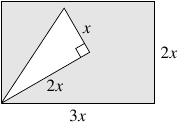
\includegraphics{ShadedArea.png}
%\begin{tikzpicture}
%\draw[fill=gray!20] (0,0) --node[below]{$3x$} (3,0) -- node[right]{$2x$} (3,2) -|(0,0);
%\draw[rotate=30,fill=white] (0,0) --node[below right=-.1cm]{$2x$} (2,0) --node[right]{$x$} (2,1) -- (0,0) (2,0) rectangle ++(-.2,.2);
%\end{tikzpicture}
\end{image}

Find a formula for each function.

\begin{hint}
The area of a rectangle is length times width.
\end{hint}
\begin{prompt}
$f(x)=$ \answer{6x^2}.
\end{prompt}

\begin{hint}
The area of a triangle is one half base times height.
\end{hint}
\begin{prompt}
$g(x)=$ \answer{x^2}.
\end{prompt}

What does the function $h(x)=f(x)-g(x)$ represent geometrically?
\begin{hint}
What do $f$ and $g$ represent? 
\end{hint}
\begin{multipleChoice}
\choice{the combined perimeter of both figures}
\choice{the area of both figures}
\choice[correct]{the area of the shaded region}
\choice{half of the total area}
\end{multipleChoice}

\begin{hint}
Remember that $h$ is the function that gives the area of the shaded region. 
\end{hint}
\begin{prompt}
$h(2)=$ \answer{20}
\end{prompt}
\end{question}

We can obtain new functions by multiplying and dividing functions as well. 
For example if $f(x)=x^2-2$ and $g(x)=x+3$ then 
\[
f(x)g(x)=[x^2-2][x+3]=[x^2-2]\cdot x+[x^2-2]\cdot 3=x^3-2x+3x^2-6,
\]
and
\[
\frac{f(x)}{g(x)}=\frac{x^2-2}{x+3}.
\]


\begin{question}
Suppose we have a rectangle whose dimensions are changing over time. Let $w(t)$ be the function that gives the width of the rectangle at time $t$ and $l(t)$ be the function that gives the length of the rectangle at time $t$.

What does the function $h(t)=w(t)l(t)$ represent geometrically?

\begin{hint}
What do you get when you multiply the length and the width of a rectangle? 
\end{hint}
\begin{multipleChoice}
\choice{the perimeter of the rectangle at time $t$}
\choice{the length of the diagonal of the rectangle at time $t$}
\choice[correct]{the area of the rectangle at time $t$}
\choice{the difference between the width and length at time $t$}
\end{multipleChoice}

\end{question}

\end{document}
